\begin{tikzpicture}[scale=\trackingExampleScale, every node/.style={transform shape}]
    \begin{scope}[baseline=(image1.south)]
        \node (image1) {
            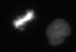
\includegraphics[width=0.25\textwidth]{images/cell_tracking/example_00.png}
        };
    \end{scope}
    \begin{scope}[baseline=(image2.south)]
        \node[right=of image1, xshift=-20pt] (image2) {
            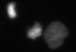
\includegraphics[width=0.25\textwidth]{images/cell_tracking/example_01.png}
        };
    \end{scope}
    \begin{scope}[baseline=(image3.south)]
        \node[right=of image2, xshift=-20pt] (image3) {
            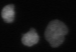
\includegraphics[width=0.25\textwidth]{images/cell_tracking/example_02.png}
        };
    \end{scope}
\end{tikzpicture}


%%% Local Variables: 
%%% mode: latex
%%% TeX-master: "../../../main"
%%% End: 
